
\subsubsection*{Условие квазистационарности}
Условие квазистационарности заключается в том, что характерное время изменения макроскопических величин (таких как ток, напряжение, частота или импеданс) в цепи должно быть сильно меньшим времени распространения сигнала в цепи (размер цепи делить на скорость света).


\subsubsection*{Зарядка и разядка конденсатора}

\begin{figure}[h]
    \centering
    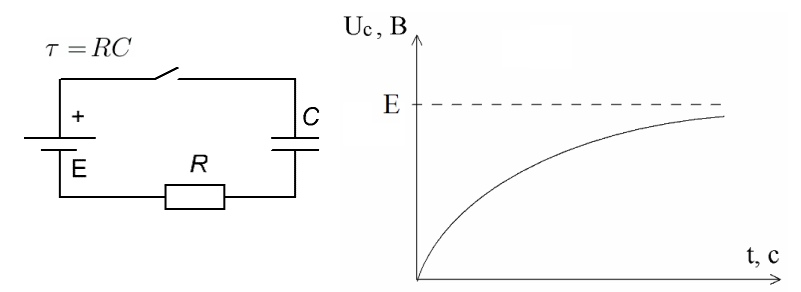
\includegraphics[width=0.5\textwidth]{img/2.jpg}
    %\caption{}
    %\label{fig:}
\end{figure}

Зарядка и разрядка конденсатора описывается следующим дифференциальным уравнением и его решением ($U_c$ -- напряжение на конденсаторе): 
$$
    E = U_c + RC\dot{U_c};
    \hspace{0.5cm} 
    U_c = E - ke^{-RCt}
$$ где $k$ - постоянная интегрирования, зависит от начального напряжения на конденсаторе, а $RC$ - характерное время зарядки конденсатора.


\subsubsection*{Установлени тока в катушке индуктивности}

Если в схеме для конденсатора заменить его на индуктивность, то получим следующее уравнение и его решение ($k$ - постоянная интегрирования, зависящая от начального тока): 
$$
    E = IR + \dot{I}L; \hspace{0.5cm} 
    I = \frac{E}{R} + ke^{-\frac{R}{L}t}; \hspace{0.5cm} 
    k = I_{\text{нач}} - \frac{E}{R}
$$


\subsubsection*{Интегрирующие и дифференцирующие цепочки}

\begin{figure}[h]
    \centering
    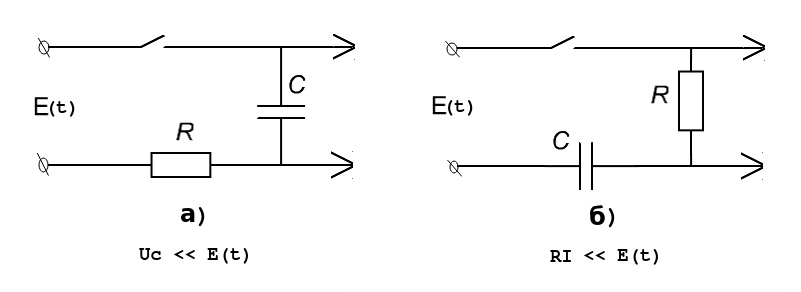
\includegraphics[width=0.5\textwidth]{img/1.jpg}
    %\caption{}
    %\label{fig:}
\end{figure}


Если в нарисованной выше схеме подавать вместо $E$ какой-то сигнал, то в случае а):
$$
    E(t) = U_c + \dot{U_c}CR \approx \dot{U_c}R;\
    \hspace{0.5cm} 
    U_c \approx \frac{1}{RC}\int E(t)dt,
$$
В случае б):
$$
    E(t) = U_c + \dot{U_c}CR \approx U_c;
    \hspace{0.5cm}  U_R \approx RC\frac{dE(t)}{dt}.
$$